
\begin{frame}
  \frametitle{Évolution des Processeurs Graphiques}
  \begin{center}
    \begin{tikzpicture}[yscale=-1]
      % \draw[help lines] (0,0) grid (15,6);
      % > latex arroxw
      \draw[line width=10pt,-latex] (1.5,1) .. controls +(1,4) and +(-5,-0) .. +(10,4);
      \node at (1.5,1) {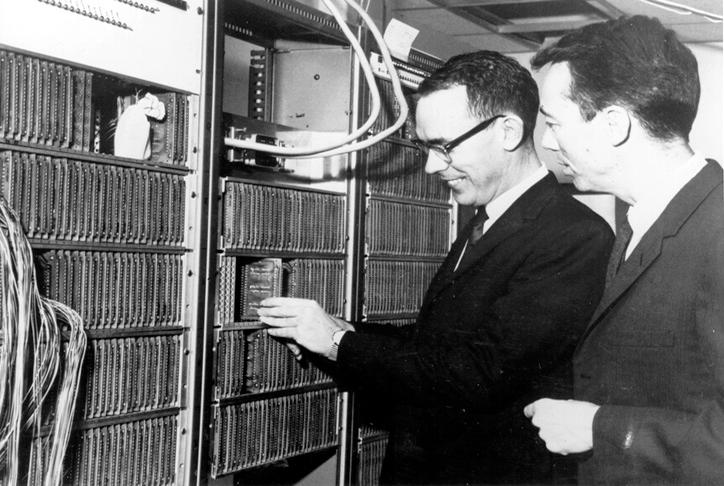
\includegraphics[scale=.1]{images/evans-sutherland.jpg}};
      \node [anchor=south] at (1.5,0) {Evan \& Sutherland};
      \node at (3,3.25) {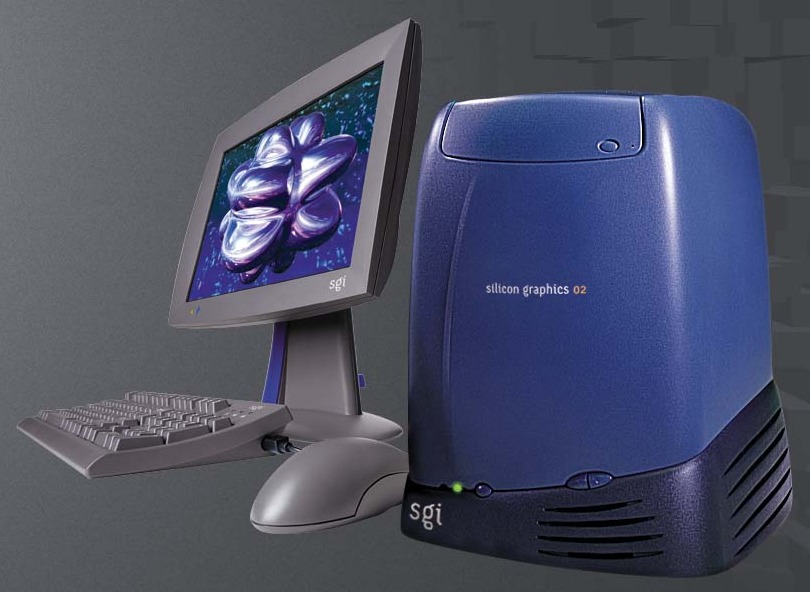
\includegraphics[scale=.1]{images/sgi-o2-workstation.jpg}};
      \node [anchor=north] at (2.5,4.25) {SGI Workstation};
      \node at (6,4.75) {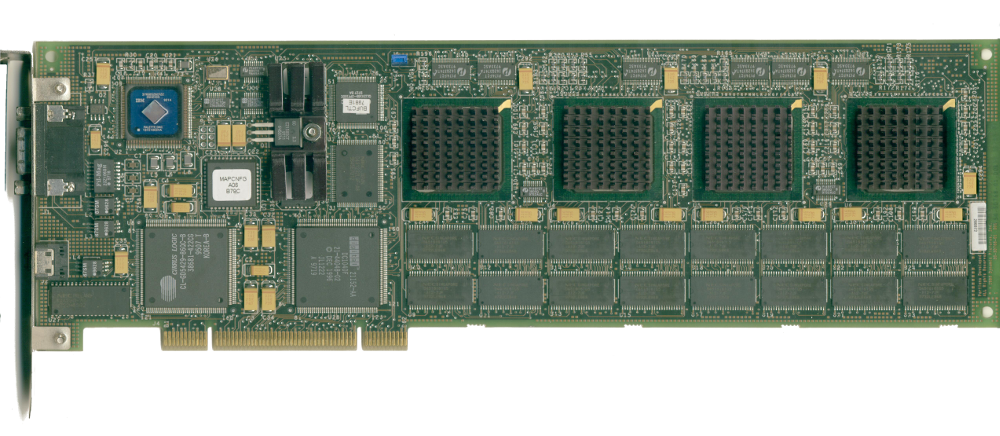
\includegraphics[scale=.5]{images/oxygen.png}};
      \node [anchor=north] at (6,5.25) {Accélerateur Graphique};
      \node at (9,5) {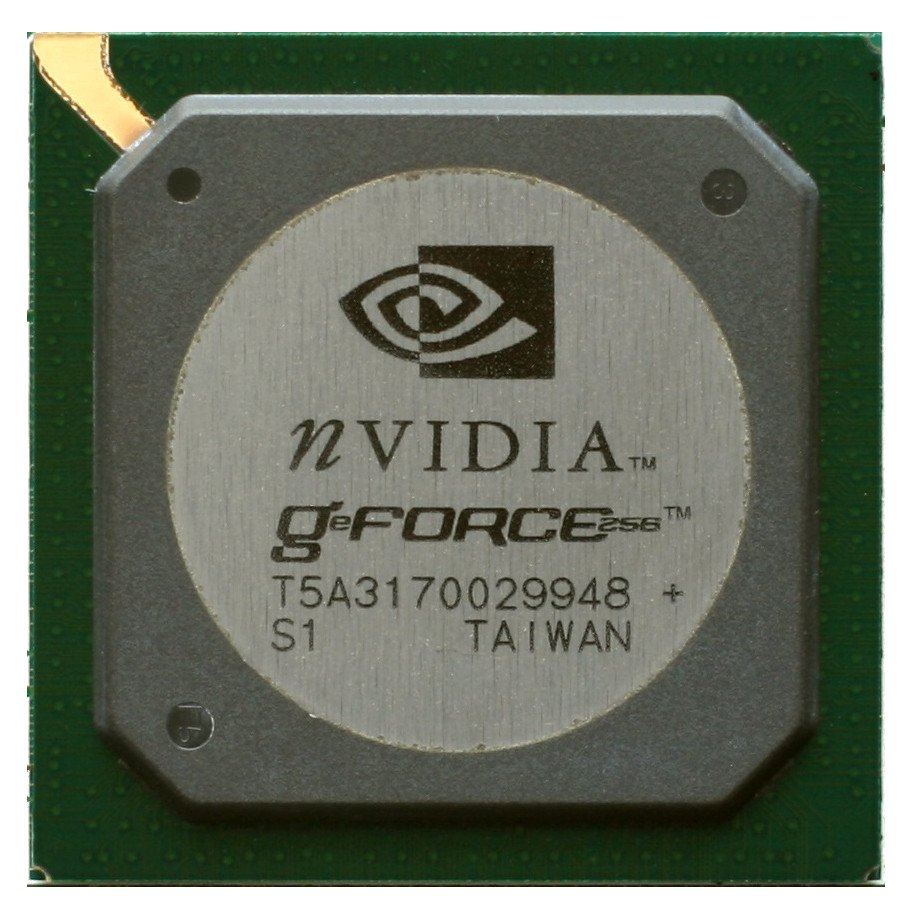
\includegraphics[scale=.03]{images/nvidia-gforce.png}};
      \node [anchor=south,align=center] at (9,4.5) {Nvidia GeForce 256\\ first GPU}; % First GPU
      \node [anchor=west,align=left] at (11.5,5) {General Purpose\\ GPU};
      \draw (14.5,0) -- +(.01,0); % hack
    \end{tikzpicture}
  \end{center}
  \begin{textblock}{12}(3.5,2.5)
    \begin{itemize}
    \item convergence du hardware professionnel et consumer
    \item convergence des processeurs graphiques et de flux
    \item convergence des plateformes~: de l'embarqué au super-calculateur 
    \end{itemize}
  \end{textblock}
 \end{frame}

\begin{frame}
  \frametitle{Présentation des GPUs: processeur de flux}
  % dessin flux de données traversant la page
  \begin{center}
    \begin{tabular}{cc}
      Intel Haswell Die & Nvidia Kepler Die \\[5mm]
      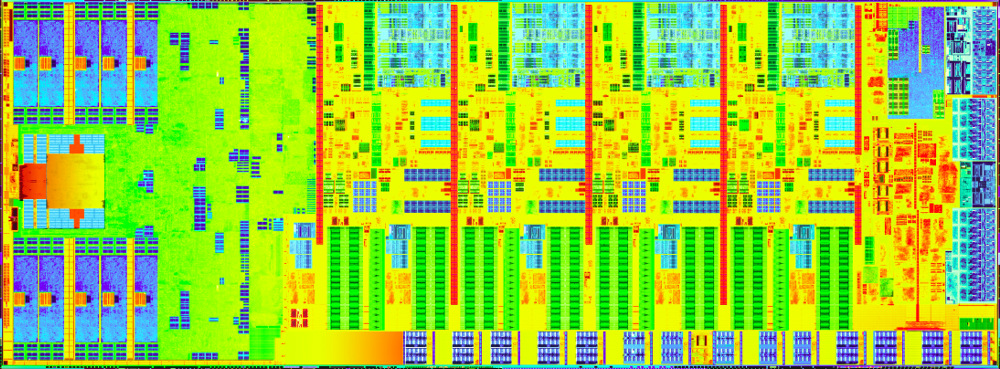
\includegraphics[height=.3\textheight]{images/intel-haswell-die.jpg} &
      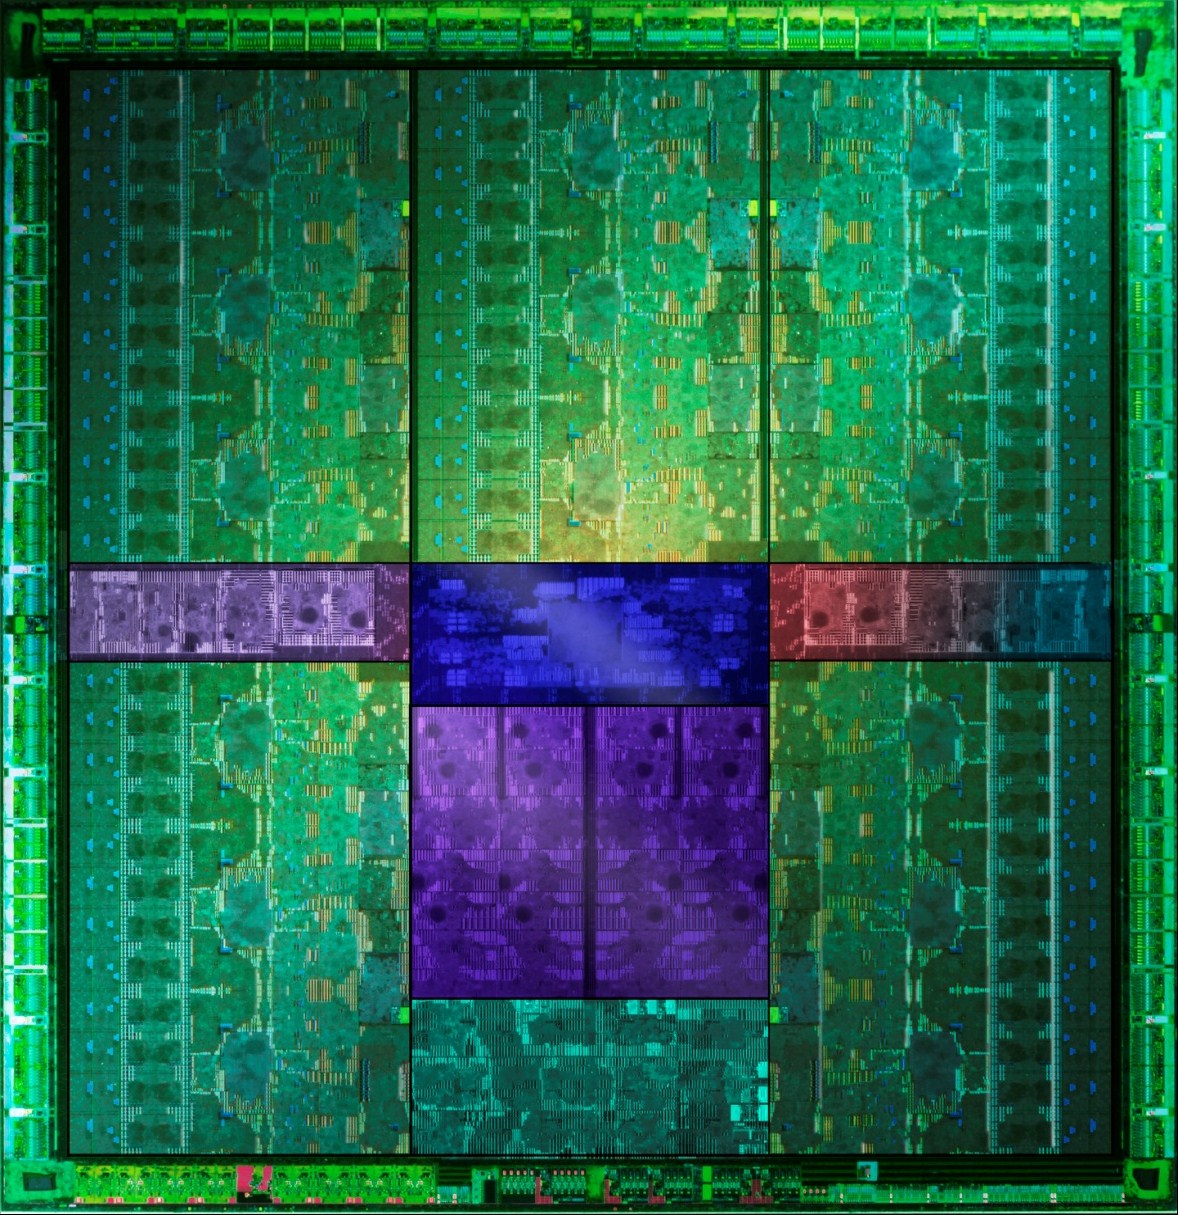
\includegraphics[height=.3\textheight]{images/nvidia-kepler-die.jpg}
    \end{tabular} \\[5mm]
    Architecture de calcule hautement parallèle \\
    couplé à une mémoire rapide (GDDR5)
  \end{center}
  \note[enumerate]
  {
  \item CPU~: usage générique
  \item SIMD AVX2 256-bit 8x float 32-bit
  }
\end{frame}

\begin{frame}
  \frametitle{Usage des GPUs}
  % keywords picture
  % pgf mindmap cf. p75
  \begin{columns}
    \begin{column}{.25\textwidth}
      \begin{center}
        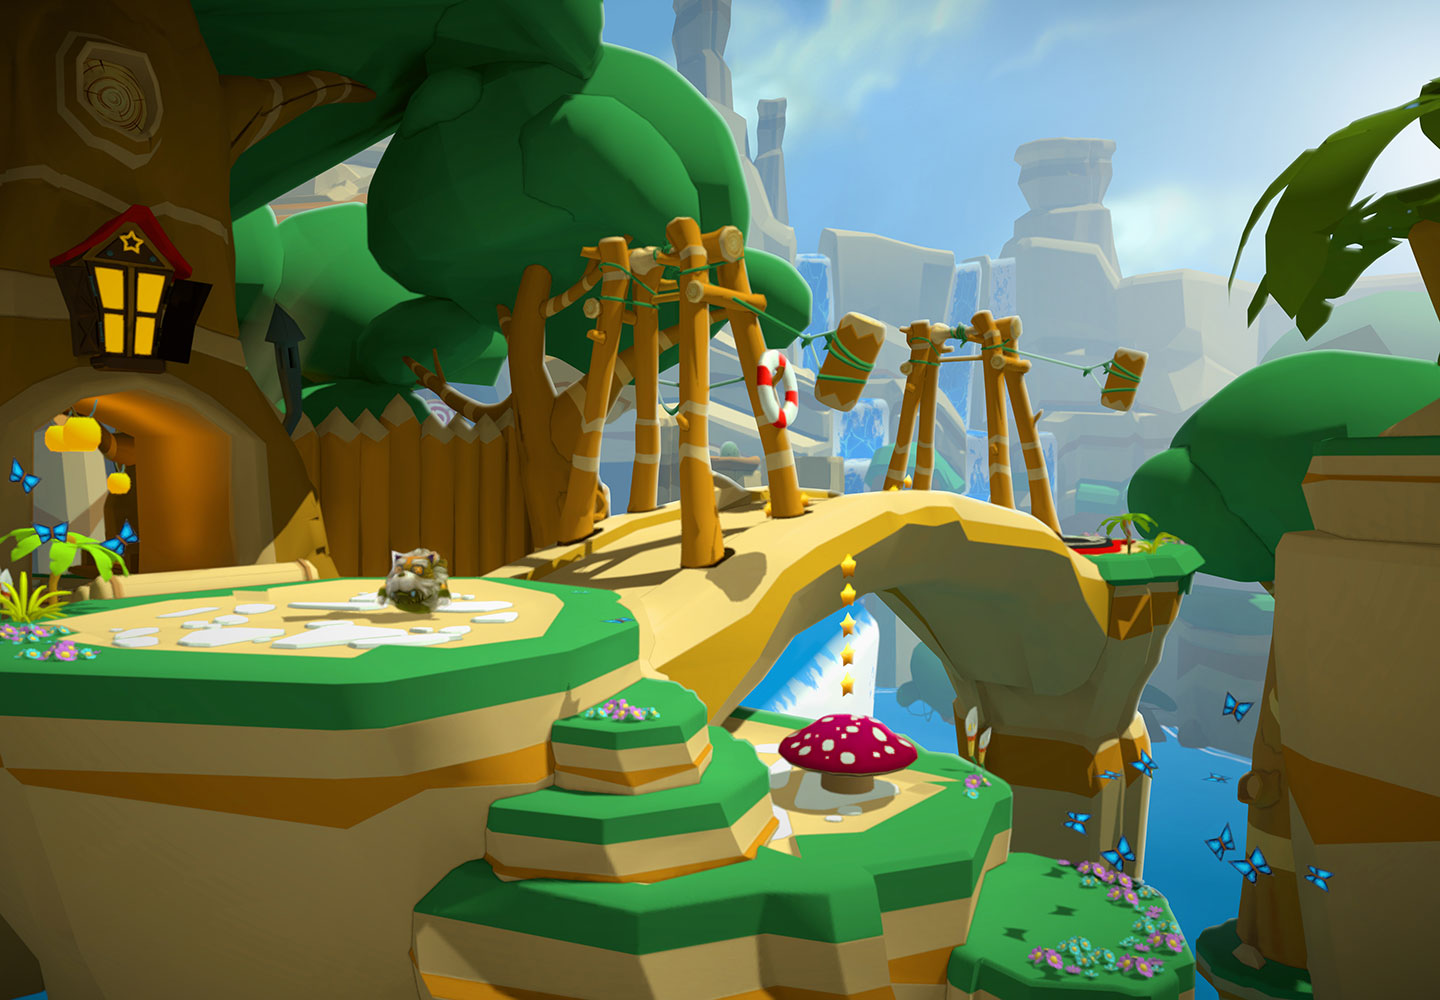
\includegraphics[width=1.\textwidth]{images/game.jpg} \\[5mm]
        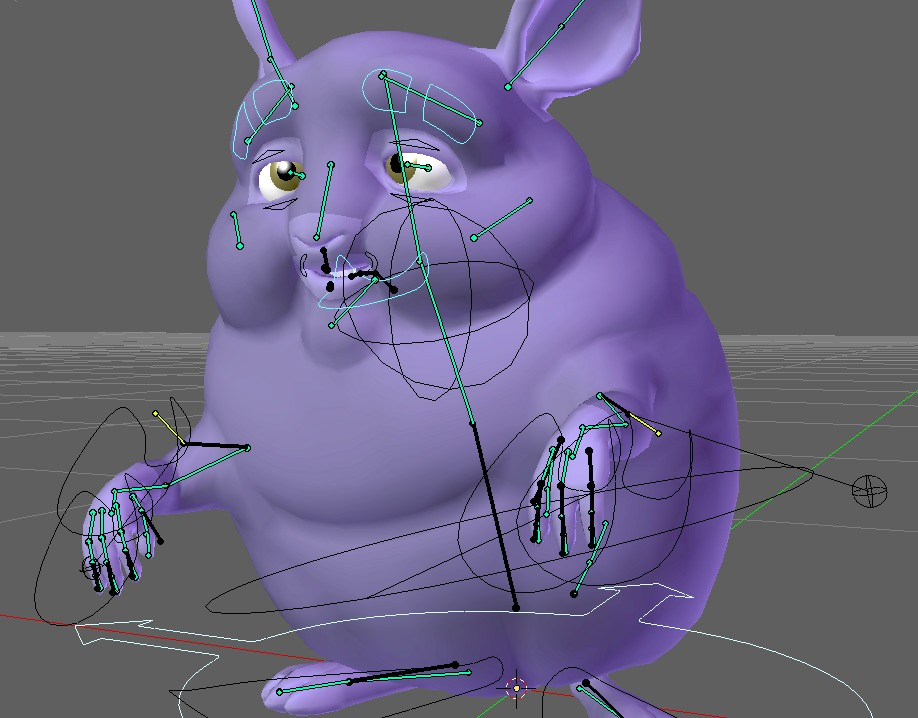
\includegraphics[width=1.\textwidth]{images/blender.jpg}
      \end{center}
    \end{column}
    \begin{column}{.25\textwidth}
      \begin{center}
        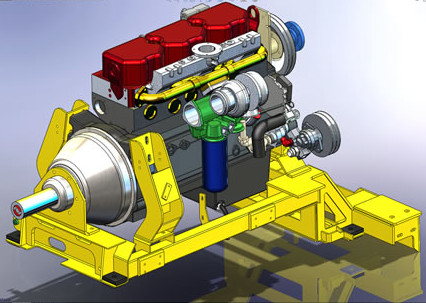
\includegraphics[width=1.\textwidth]{images/solidworks.jpg} \\[5mm]
        
\includegraphics[width=.8\textwidth]{images/tiger.jpg}
      \end{center}
    \end{column}
    \begin{column}{.5\textwidth}
      \begin{itemize}
      \item Moteur de jeu % Game Engine
      \item Modeleur \textbf{3D}
      \item CAO
      \item \textbf{Visualisation} scientifique
      \item \textbf{Interface graphique} \\
        e.g.\ Qt QML, KDE Plasma
      \item \textbf{2D} avec accélération matériel
      \item \textbf{Calcul}~: CUDA, OpenCL
      \end{itemize}
    \end{column}
  \end{columns}
  \note[enumerate]
  {
  \item \url{https://developer.nvidia.com/nv-path-rendering} \\
    KILGARD, M., AND BOLZ, J. 2012. GPU-accelerated path rendering. ACM Transactions on Graphics
    (Proceedings of SIGGRAPH Asia 2012) 31, 6. 106
  \item Shader-based Antialiased Dashed Stroked Polylines \\
    N. P. Rougier. Journal of Computer Graphics Techniques, 2.2 (2013). \\
    \url{http://jcgt.org/published/0002/02/08/}
  \item Higher Quality 2D Text Rendering \\
    N. P. Rougier. Journal of Computer Graphics Techniques, 2.1 (2013). \\
    \url{http://jcgt.org/published/0002/01/04/}
  \item OpenVG, SVG, Display Postscript
  }
\end{frame}

\begin{frame}
  \frametitle{Présentation de l'API OpenGL}
  \begin{columns}
    \begin{column}{.2\textwidth}
      \begin{center}
        
\includegraphics[width=1.\textwidth]{images/khronos-logos/OpenGL/OpenGL_500.jpg} \\
        
\includegraphics[width=1.\textwidth]{images/khronos-logos/OpenGL_ES/OpenGL-ES_500.jpg} \\
        
\includegraphics[width=1.\textwidth]{images/khronos-logos/WebGL/WebGL_500.jpg} \\
        
\includegraphics[width=1.\textwidth]{images/khronos-logos/Khronos_Group/Khronos_Group_500.jpg}
      \end{center}
    \end{column}
    \begin{column}{.8\textwidth}
      \begin{itemize}
        \item Un standard ouvert géré par le groupe Khronos
        \item La seule API cross-platforme et cross-vendor
        \item L'API de facto de GNU/Linux et d'Android
        \item Une API orientée desktop (OpenGL) et embarqué (OpenGL ES)
        \item mais aussi orientée web (WebGL)
      \end{itemize}
    \end{column}
  \end{columns}
\end{frame}

\begin{frame}
  \frametitle{Évolution de l'API OpenGL}
  \begin{center}
    \includegraphics[width=.6\textwidth]{figures/opengl-release-date.pdf} % ,transparent
  \end{center}
  \note[enumerate]
  {
  \item 20 ans
  \item dynamique des releases
  }
\end{frame}

\begin{frame}
  \frametitle{Programmable Pipeline}
\end{frame}

\begin{frame}
  \frametitle{Implémentations}
  \begin{center}
    \includegraphics[width=.6\textwidth]{figures/mesa-status.pdf} % ,transparent
  \end{center}
\end{frame}

\begin{frame}
  \frametitle{Python interfaces}
  \begin{itemize}
    \item PyOpenGL
    \item pyglet~: a cross-platform windowing and multimedia library
    \item Vispy~: a high-performance interactive 2D/3D data visualization library
  \end{itemize}
  \note[enumerate]
  {
  \item http://pyopengl.sourceforge.net
  \item http://www.pyglet.org
  \item http://vispy.org
  }
\end{frame}

\begin{frame}
  \frametitle{PyOpenGL}
\end{frame}

%%% Local Variables: 
%%% mode: latex
%%% TeX-master: "master"
%%% End: 
